\chapter {Functional requirements}

The functional requirements are based on the non-functional requirements. Additional requirements are derived from the technical environment and its specifications. \\
\\
To be able to display the data of Wikidata, ArticlePlaceholder are based on Wikibase and MediaWiki. \\
As MediaWiki is written in PHP, the main part of the extension has to make use of that language and the services provided by MediaWiki and Wikibase. \\
The programming language for scripts on Wikipedia is Lua. Therefore the parts that will be user-editable are written in Lua, so they can be overwritten by the local communities. \\
The default for the content pages presents the information and data in a useful way, and to make it visually appealing, it should make use of images when possible. \\
For users without access to a computer (as in the scenario of Edha) the layout of the extension is required to be responsive and work on mobile devices. \\
Some of the following requirements are scheduled for later implementation during the course of the project. 

\section{Naming}
Since the users need to be able to find the ArticlePlaceholder easily it is implemented as a SpecialPage. This SpecialPage should have a short name that is convenient to remember. Therefore it is called \textit{AboutTopic}.

\section{Display ArticlePlaceholder}
The pages displaying the content of a Wikidata item focus on a clear differentiation between the layout of the ArticlePlaceholder and what a user-written article looks like. They still contain elements of the well-known Wikipedia layout to appeal to readers and fit in with the other content as the references at the bottom. \\
A default layout is needed, but it is important to give the user control over every part of the page. In doing so, users such as Julian are enabled to adjust the layout to their communities' needs.

\section{Internationalization}
It is important to have the whole extension ready to be localized from the beginning. This is necessary for the extension to be used by an international community. \\ 
\begin{quote}
``Internationalization refers to the adaptation of products to support or enable localization for international markets. Key features of internationalization have always been the support of international natural language character sets, separation of locale-specific features such as translatable strings from the software code base and the addition of functionality or features specific to foreign markets. Without internationalization, localizing a product can be very challenging'' states \citet[23]{localization}. 
\end{quote}
Since the data on Wikidata is multilingual, this focuses more on aspects like labels on buttons and the name of the SpecialPage itself.

\section{Discover ArticlePlaceholder}

There are multiple ways for a reader to get to an ArticlePlaceholder. 

\subsection{SpecialPage URL}
Beside the input form of the SpecialPage there should be a way to directly link to an ArticlePlaceholder page as users as Heather would require.

\subsection{Search}
In order to get to an ArticlePlaceholder while looking for a topic, the generated pages are added to the search on Wikipedia. There are different possible positions for the results in the search page. They could be attached to the bottom of the results, or placed to the right of the regular search results. \\
\\
It is important to point out that the notability criterias on a Wikipedia are not necessarily the same as on Wikidata. The results in the search should be limited to notable items. \\
Showing only notable items is especially important since article creation should only be encouraged when it makes sense. This avoids the creation of articles, that would be deleted by other users later on. Otherwise the community building and trust the ArticlePlaceholer is supposed to be working on would be compromised. \\
Since it is hard to decide which content is actually notable, the items appearing in the search should be limited to the ones having at least one statements and two sitelinks to the same project (like Wikipedia or Wikivoyage). \\
\\
Catrin's scenario shows how a user would start their research with an ArticlePlaceholder. Therefore whenever possible the ArticlePlaceholder should link to existing Wikipedia articles. Due to the limitation of the data received from Wikidata, this is not in the scope of this thesis. \\
\\
Many users will research information on web search engines such as Google and arrive at Wikipedia from the result page. In order to make the data provided by the ArticlePlaceholder accessible for those users, it will be necessary for the generated pages to be indexable.
\begin{figure}[H]
	\centering
	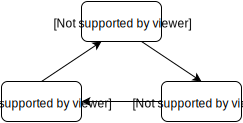
\includegraphics[width=80mm]{diagrams/CircleSearchAttention.png}
	\caption{Problem for small Wikipedias}
	\label{fig:CircleSearch}
\end{figure}
As described in Figure~\ref{fig:CircleSearch} a problem of the small Wikipedia projects is being stuck in a vicious circle: Since they have few articles, they do not receive a lot of attention via search engines such as Google, so they are not able to attract new editors and therefore they do not consist of many articles. \\
\\
Making ArticlePlaceholder accessible for search engines will be an important point in the following development of the extension. 

\subsection{Red links}
\begin{quotation}
``A red link (...) signifies a link to a page that is either non-existent or deleted.'' \citep{wiki:01} 
\end{quotation}

Red links are used frequently in Wikipedia to indicate an article which is does not yet exist, but should. Today it leads the user to an empty \textit{create article} page. In the future it should instead bring them to an ArticlePlaceholder, offering the option of creating an article. This is part of the topic of \textit{smart red links}, which is discussed in the section~\ref{sec:redLinks}: \nameref{sec:redLinks}.

\section{Article creation}
Starting at the ArticlePlaceholder created by the extension, the user may want to create an article to provide more information and give this data a context that only natural language can provide. \\
Two different strategies are in consideration at the moment: Creating an article from scratch, or translating an existing article into the user's language. \\
The challenge is to encourage editors to add a new article if appropriate, and at the same time prevent vandalism such as ``any addition, removal, or change of content, in a deliberate attempt to damage Wikipedia. Examples of typical vandalism are adding irrelevant obscenities and crude humor to a page, illegitimately blanking pages, and inserting obvious nonsense into a page.'' \citep{wiki:33} \\ 
The title for the article they want to create might differ from the label of the item, due to the local Wikipedia's rules and customs. Therefore a user must be able to enter a title for the page that does not exist on that Wikipedia yet. \\
After entering the title of the new article, the user is redirected to an empty editing page, where they can add their content. \\
In the future it is intended to add the data provided by Wikidata to the editing page so the user can use it while writing the article. 

\subsection{Content translation}
Using the content translation tool\footnote{\url{https://www.mediawiki.org/wiki/Content_translation}}, the user should be able to translate an article from an existing one in another language. This is not within the scope of this thesis; the focus for now is to create articles from scratch. \\

\section{Ordering of statement groups}
The data in Wikidata is not ordered in a meaningful manner. ArticlePlaceholder aims at readers looking for an overview of the topic and therefore only need the most important data on a topic. \\
\\
To keep the editors in control, there should be a list of properties maintained on-wiki. They are ordered by their importance. \\
The ordered list includes labels of the properties as well as their numbers for users unfamiliar with Wikidata. The list can be annotated with comments on each line to provide additional information and help other editors understand the context of the property and its position in the ordered page. \\
This list is only editable by administrators on the Wikipedia so as to reduce constant changing of the displayed information. \\
This list is then used to order and filter the statements on each ArticlePlaceholder page. 

\section {Identifier}
Identifiers are IDs used for an entity in other ontologies. For the reader to be able to conveniently look up more information on sites other than Wikimedia projects, identifiers need to be distinguishable from other statements also in the layout, and always show up on the ArticlePlaceholder. To always be displayed, they should not be included in the list of ordered statements. 

\section{Caching}
Since the generated content pages will be accessed frequently, it will be necessary to implement some form of caching for them. In Figure~\ref{fig:pageviews} is an example for the page views per day of the English Wikipedia's \textit{MainPage} to emphasize how urgent the need for caching will be. \\
With caching it would be possible to limit the amount of requests to Wikidata services too, which will show an improvement in the performance. This is not part of this thesis.

\section {Unit tests}
It is especially important for the main code in PHP to be covered completely by automated testing, especially by unit tests. \\
It is necessary to set up continuous integration in a way that is integrated with MediaWiki and Wikibase. Then the code will conform to coding conventions, but also allows for running the unit tests automatically. This will reduce the time spent on code reviews, testing and bug fixing. \\
This has been done in cooperation with the Wikidata team while working on the extension. Neither the integration tests nor the tests for the Lua code are covered in this thesis. \\ 